\documentclass[asp1.tex]{subfiles}
\begin{document}

\section{Prüfungsvorbereitung}

\subsection{Begriffe aus dem Lernfeld}

\begin{longtable}{|p{.2\textwidth}|p{.8\textwidth}|}
        \hline

        \textbf{Begriff} & \textbf{Erläuterung} \\\hline

        \textbf{SLA (Service Level Agreements)} &

        Ein Service Level Agreement (SLA) ist ein Vertrag zwischen einem Dienstleistungsanbieter und seinen Kunden, der dokumentiert, welche Dienstleistungen der Anbieter erbringen wird, und der die Dienstleistungsstandards definiert, zu deren Einhaltung der Anbieter verpflichtet ist.

        Beinhaltet z.B.:
        \begin{outline}
            \1 die Verfügbarkeit (Berechnung aus dem 1. Lehrjahr)
            \1 Servicebereitschaft von wann bis wann
            \1 Reaktionszeit auf Störungen und maximale Dauer bis zur Entstörung
            \1 Ggf. Hinweise zum Monitoring von Produkten
        \end{outline}
        \\\hline

        \textbf{Ticketsystem} &
        Ein Ticketsystem ist ein Ordnungssystem. Es behandelt systematisch entweder von Kunden oder der eigenen Belegschaft formulierte Probleme mit einem Produkt oder einer Dienstleistung.

        Ticketsysteme werden am häufigsten im Kundensupport eingesetzt.

        Die Support Tickets werden kategorisiert, ihnen werden Prioritäten zugewiesen und sie werden zur passenden Bearbeitungsstelle weitergeleitet. Der beauftragte Mitarbeiter kann durch Verknüpfung mit der Kundendatenbank auf alle früheren Anfragen des Kunden über alle Kanäle zugreifen.

        Produkte sind z.B. Servicenow, Jira Service Desk, Happy Fox
        \\\hline

        \textbf{First-Level-Support} &
        Ein First-Level-Supporter ist der erste Ansprechpartner für Beratung und Hilfe im IT- und Computerbereich.

        Wenn der First-Level-Supporter kontaktiert wird, trägt er zunächst die Daten des Kunden, alle eingehenden Anfragen und weitergehende Informationen zusammen. Anschließend listet er sie auf. Die Dokumentation sollte möglichst lückenlos erfolgen, um unangenehme Nachfragen beim Kunden und eine reibungslose Weitergabe der Anfrage an den nächsten Support-Level zu gewährleisten. Zunächst kümmert sich aber der First-Level-Supporter eigenständig um das Problem. Neben seiner Erfahrung kann er bei Bedarf auch das Wissen externer Datenbanken zu Rate ziehen. In dieser Phase erfolgt daneben auch eine Einstufung der Probleme, die die Kunden haben.
        \\\hline

        \textbf{Second-Level-Support}
        \textbf{Third-Level-Support}
        &
        Der Second-Level-Support ist die zweite Ebene im Kundenservice eines Unternehmens. Beim Second-Level-Support kommt es darauf an, Probleme technischer Art beim Kunden mit seinem Gerät in der Regel quasi per Ferndiagnose am Telefon oder per Internet-Online Support zeitnah zu lösen.

        2nd Level Supporter müssen über entsprechendes Fachwissen verfügen, was bei 1st Level Support nicht zwingend erforderlich ist.

        Im Third-Level-Support werden entsprechend der Klassifizierung ausschließlich Experten und Spezialisten eingesetzt. Diese Stufe wird nur eskaliert, wenn der 2nd Level keine Lösung gefunden hat.
        \\\hline

        \textbf{IT-Service Desk}&
        Der Service Desk ist die \textbf{Kommunikationszentrale}, die als einzige Schnittstelle (Single Point of Contact, kurz SPOC) zwischen dem Service-Nehmer und dem Service-Geber dient. Die Sicherstellung und eine angemessene schnelle Hilfe mit fest definierten Service Level Agreements bereit stellen zu können, ist der Zweck eines \textbf{IT-Service Desk}.

        Der Service Desk deckt eine große Bandbreite an Aufgaben ab und ist so konzipiert, dass er als alleinige Anlaufstelle des Anwenders für all dessen IT-Anforderungen fungieren kann. Damit spielt der Service Desk eine zentrale Rolle bei der Integration von Geschäftsprozessen mit dem Technologie-Ökosystem und der breiteren Service-Management-Infrastruktur.
        \\\hline

        \textbf{Helpdesk}&
        Ein Helpdesk, Help-Desk oder User-Help-Desk (UHD) ist ein Issue-Tracking-System, das vorrangig für die Unterstützung von Anwendern von Hard- und Software, aber auch für Anfragen von Kunden in anderen Dienstleistungsbereichen zuständig ist.

        Die Hilfe (Help) kann dabei über klassischen Telefonservice, aber auch mit Hilfe technischer Geräte sowie von Software (Fernwartung, Live-Support-System) erfolgen.

        In speziellen Issue-Tracking-Systemen werden die Anfragen verwaltet. Damit kann einerseits von allen eingesetzten Kundenbetreuern auf die Service- und Fehlerhistorie zurückgegriffen und andererseits durch Fehleranalysen die Weiterentwicklung der Produkte oder des Service unterstützt werden.
        \\\hline

        \textbf{ITIL (Information Technology Infrastructure Library)}&
        Best-Practice-Leitfaden und der De-facto-Standard im Bereich IT-Service-Management. ITIL besteht nicht aus starren Vorgaben, sondern ist vielmehr eine \textbf{Sammlung von Leitlinien}, die an die Anforderungen einzelner Unternehmen angepasst werden können.

        Beispielhafte Prozesse: \newline
        \href{https://wiki.de.it-processmaps.com/index.php/Incident_Management}{Incident Management} \newline
        \href{https://wiki.de.it-processmaps.com/index.php/Problem_Management}{Problem Management} \newline
        \href{https://wiki.de.it-processmaps.com/index.php/Change_Management}{Change-Management}
        \\\hline

        \textbf{Service Request (ITIL)}&
        Service Request ist eine formale Anfrage eines Anwenders nach etwas, das bereitgestellt werden soll, beispielsweise eine Anfrage nach Informationen oder Beratung, danach ein Passwort zurückzusetzen oder einen Arbeitsplatz für einen neuen Anwender zu installieren.
        \begin{outline}
            \1 Eine formale Anfrage eines Anwenders - z.B. nach Informationen, Beratung, Zurücksetzen eines Passworts, oder Installation einer Workstation für einen neuen Benutzer.
        \end{outline}
        \\\hline

        \textbf{Event (ITIL)}&
        Eine Statusänderung sowie ein Alarm oder eine Benachrichtigung, die durch einen IT-Service, ein Configuration Item oder ein Überwachungstool erzeugt wurde.

        Z.B. „Weniger als 10% Speicherkapazität steht zur Verfügung.“
        \\\hline

        \textbf{Incident (ITIL)}&
        Ein Incident ist eine Beeinträchtigung oder Unterbrechung eines angebotenen Service. Eine Beeinträchtigung liegt dann vor, wenn der Service nach der Vereinbarung zwischen Servicegeber und Servicenehmer (SLA) quantitativ oder qualitativ nicht wie vereinbart genutzt werden kann.

        Z.B. „Ein Kunde meldet, dass Druckaufträge nicht verarbeitet werden.“
        \\\hline

        \textbf{Remote-Support}&
        Remote-Support-Software ermöglicht es IT-Technikern, aus der Ferne auf einen anderen Computer oder ein anderes Gerät zuzugreifen, um Support zu leisten.

        Dies geschieht meist über eine VPN-Software wie z.B. TeamViewer
        \\\hline

        \textbf{GS-Zeichen}&
        Das GS-Zeichen bestätigt die Konformität mit dem Gerätesicherheitsgesetz. Es ist ein in Deutschland gültiges nationales Kennzeichen.

        
\includegraphics{gs.jpg}
        \\\hline

        \textbf{VDE Zeichen}&
        Das VDE-Zeichen dokumentiert die Sicherheit und Normenkonformität eines elektrotechnischen Erzeugnisses hinsichtlich elektrischer, mechanischer, thermischer, toxischer und sonstiger Gefährdungen. Es wird ausschließlich vom VDE Prüf- und Zertifizierungsinstitut vergeben. Ein Hersteller darf seine Produkte nur nach erfolgter Überprüfung und Ausstellung eines entsprechenden Zertikates mit dem VDE-Zeichen versehen.

        
\includegraphics{vde.png}
        \\\hline

        \textbf{CE Zeichen}&
        Das CE-Kennzeichen ist kein Prüfzeichen. Es ist ein Verwaltungskennzeichen und dokumentiert die Konformität des Produktes mit den geltenden EG-Richtlinien. Damit erklärt der Hersteller des Produktes eigenverantwortlich, dass Anforderungen europäischer Richtlinien erfüllt sind. Ohne CE-Kennzeichen darf innerhalb der Europäischen Union kein Produkt in Umlauf gebracht werden.

        
\includegraphics{ce.png}
        \\\hline

        \textbf{RoHS}&
        Mit \textbf{RoHS} bezeichnet man eine EG-Richtlinie 2002/95/EG, mit der die Verwendung gefährlicher Stoffe in Elektro- oder Elektronikgeräten beschränkt werden soll. \textbf{RoHS} steht dabei als Abkürzung für das englische Restriction of (the use of certain) hazardous substances.
        \\\hline

        \textbf{Blauer Engel}&
        Der \textbf{Blaue Engel} ist das Umweltzeichen der Bundesregierung. Es garantiert "hohe Standards zum Schutz unserer Umwelt und Gesundheit - unabhängig und glaubwürdig", so Bundesumweltministerin Svenja Schulze. Die Kriterien für die Vergabe legt das Umweltbundesamt fest.

        
\includegraphics{blauer-engel.png}
        \\\hline

        \textbf{Infrastructure as a Service}&
        Bei Infrastructure as a Service stellt der Cloud Provider dem Nutzer die Infrastruktur eines kompletten Rechenzentrums bereit, z. B. in Form von:
        \begin{outline}
            \1 Rechen-, Netz- und Serverkapazität
            \1 einer Bereitstellung von Kommunikationsgeräten, wie z. B. Router oder Switch
            \1 Firewalls
            \1 Speicherplatz
            \1 von Systemen zur Sicherung bzw. Archivierung von Daten (Backup-Systeme)
        \end{outline}
        Das Unternehmen kann über eine Internetverbindung auf die gehostete Infrastruktur zugreifen und diese nutzen.
        \\\hline

        \textbf{Software-as-a-Service (SaaS)}&
        Neben Infrastructure as a Service (IaaS) und Platform as a Service (PaaS) zählt Software as a Service (SaaS) zu den populärsten Formen des Cloud Computing. Kunden können über das Internet auf Angebote zugreifen, die von einem Service-Provider gehostet werden. Die beliebtesten SaaS-Applikationen im Business-Bereich sind zum Beispiel Googles G Suite und Microsoft Office 365. SaaS-Applikationen haben sich angesichts des einfachen Zugriffs bereits in vielen Bereichen etabliert.

        Wie bei anderen Cloud-Diensten bezahlen Organisationen auch für SaaS-Anwendungen normalerweise monatlich oder jährlich eine Gebühr. SaaS-Provider rechnen Anwendungen in der Regel anhand bestimmter Nutzungsparameter ab, wie zum Beispiel der Anzahl der Personen, die die Anwendungen nutzen oder der Anzahl der Transaktionen.

        Vorteile von SaaS und IaaS sind meist eine höhere Flexibilität, geringerer Wartungsaufwand und Arbeitsaufwand und die Versorgung mit aktuellen Produkten und Dienstleistungen.

        Nachteil sind häufig der Datenschutz, langfristige Kostenstrukturen und Flexibilität der Soft- und Hardware. Diese kann häufig nicht direkt an den Kunden angepasst werden.


        \\\hline
\end{longtable}

\break

\subsection{Relevante Prüfungsaufgaben}

\subsubsection{WLAN (Sommer 2022, IT2 2.2) – Mit Lösung}

\textbf{Aufgabe:}
Bei der Einbindung der mobilen Geräte bemängelt der Geschäftsführer der InnovativFinanz GmbH, dass das WLAN sehr träge sei. Der Kunde beauftragt Sie daher mit der Messung der Datenübertragungsrate.
Ihr Ergebnis:
Die Datenübertragungsrate im WLAN erreicht ca. 50 \% der angegebenen Übertragungsrate nach IEEE 802.11.
Die Datenübertragungsrate im kupferverkabelten LAN erreicht ca. 94 %.
Beurteilen Sie diesen Sachverhalt.

\textbf{Lösung:}
Beim WLAN reduziert sich die Nettoübertragungsrate um 50\%. Das entsteht durch die falsche Koordination der WLAN-Clients durch Accesspoints oder durch räumliche Hindernisse oder durch WLAN Repeater Betrieb oder durch Fremde Funksysteme im Frequenzbereich (z.B. weitere WLANs).

Bei Verbindungen im LAN entsteht ein Protokolloverhead von ca. 6\% für Protokolldaten/Steuerdaten


\subsubsection{Anforderungsanalyse (Sommer 2022, IT1 1.1) – Mit Lösung}

\textbf{Aufgabe:}
Die Systemhaus KG berät Kunden und Kundinnen bei Fragen rund um die Themen Digitalisierung, IT-Infrastruktur und IT-Sicherheit. Sie bietet ihrer Kundschaft IT-Komplettlösungen, beginnend beider Bedarfsplanung bis zur Konfiguration und Wartung der IT-Komponenten, sowie Software an.
Die InnovativFinanz GmbH (Finanzdienstleistungsunternehmen) baut seinen Standort aus und beauftragt die Systemhaus KG, die neuen Arbeitsplätze mit Geräten auszustatten sowie die Netzwerkinfrastruktur anzupassen.
Sie sind bei der Systemhaus KG beschäftigt und bereiten die Abwicklung des Auftrages vor.

Arbeiten Sie die Kundenanforderungen aus der Anfrage (Anlage 1) heraus. Übertragen Sie diese in die unternehmensinterne Checkliste (Anlage 2).

\textbf{Anlage 1:}
Anfrage bzgl. Ausstattung Standorterweiterung Anhang:

Für unsere Niederlassung werden neue Endgeräte benötigt. Der Standort wird als Share-Place genutzt. Das bedeutet, die
12 Beschäftigten teilen sich 6 Arbeitsplätze. Die Mitarbeitenden stimmen sich untereinander ab, so dass die Arbeitsplätze innerhalb der Arbeitswoche voll besetzt sind. Die übrige Zeit sind die Kollegen und Kolleginnen bei Kunden bzw. arbeiten von zu Hause. Jeder Mitarbeitende erhält sein eigenes Endgerät.
Es ist wichtig, dass das Endgerät schnell und einfach mit 2 Monitoren verbunden werden kann. Umständliche Steckverbindungen sollten vermieden werden. Die Monitore müssen
ebenso angeschafft werden. Es sollen zwei 24 Zoll Full-HD Monitore sein, die ergonomisch im Raum platziert und justiert werden können. Alle Geräte sollten möglichst leise sein. Hier sollte auch auf den Energiebedarf und die Wärmeentwicklung geachtet werden.
Die Mitarbeitenden arbeiten primär mit Office-Anwendungen und müssen im Internet recherchieren können. Hausintern verfügen wir über ein LAN mit einer Übertragungsrate von
1 Gbit/s und über ein WLAN. Der Großteil der Daten wird auf unserem bereits vorhandenen Datei-Server abgelegt, weshalb kein großer lokaler Massenspeicher benötigt wird. Das Gerät soll schnell booten und die Anwendungen starten können. Unsere Server laufen auf Linux-Basis, die Clients sind aber Windows-Systeme. Video-Konferenzen sollen möglich sein.
Da die Mitarbeitenden neben dem Homeoffice das Gerät auch auf längeren Zugfahrten und für einzelne Kundengespräche vor Ort benötigen, muss das Gerät über einen eigenen mobilen Netzzugang verfügen. Besondere Prozessor-Leistungen oder Arbeitsspeichergrößen werden nicht benötigt. Es soll aber eine ungefähre Größenordnung angegeben werden.
Preislich planen wir mit ca. 1.500 EUR pro Mitarbeitenden.

\break

\textbf{Lösung:}
\begin{figure}[H]
    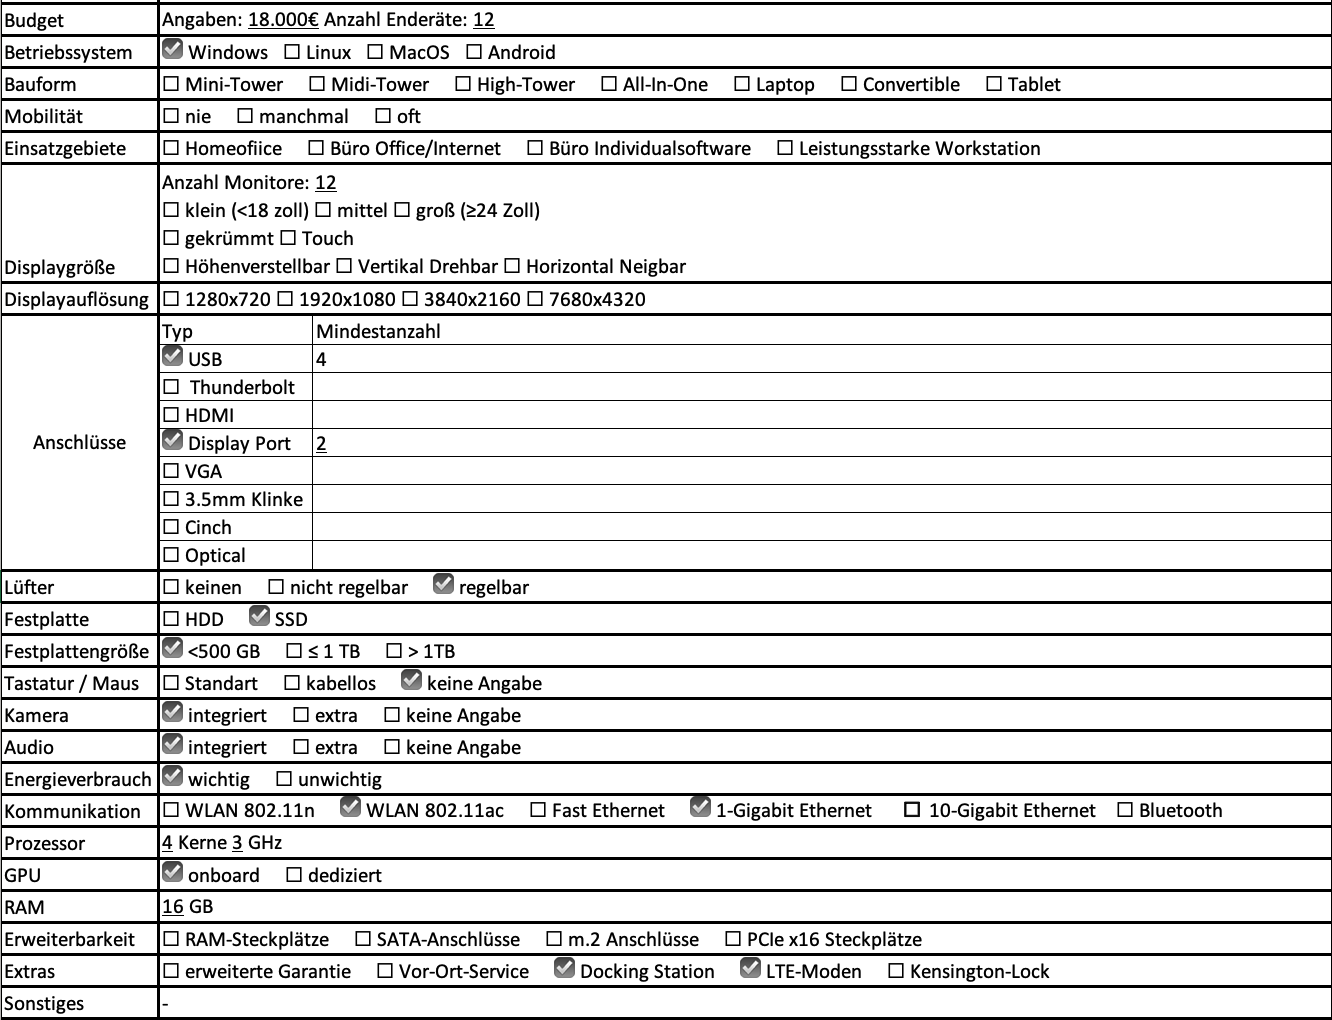
\includegraphics[width=\textwidth]{solution-excel.png}
\end{figure}

\end{document}